\subsection{The Investment and dealer Function In Financial-services Management Ch4\&8}




\subsubsection{Investments: the crossroads account}
\begin{figure}[H]
    \centering
    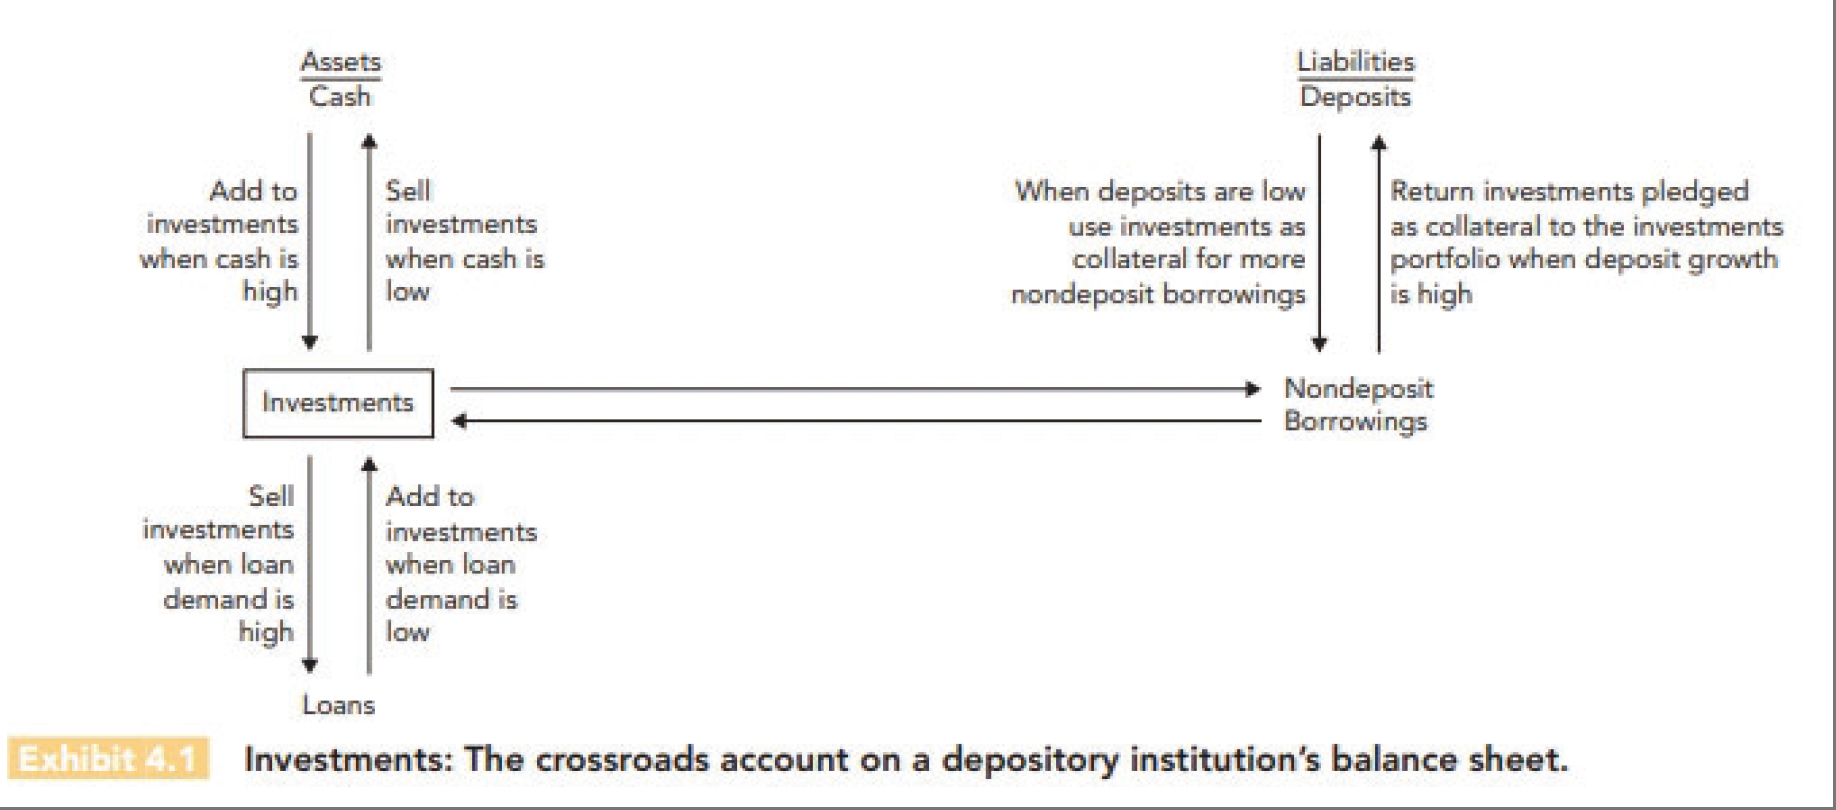
\includegraphics[width=0.5\textwidth]{images/instrument.png}
    \caption{instrument}
    \label{fig:labe18}
\end{figure}


\subsubsection{Investment instruments}
\begin{itemize}
\item To examine the different investment vehicles available, divide into two broad groups:
    \begin{itemize}
    \item Money market instruments: maturity within one year , low risk and ready marketability.
    \item Capital market instruments: maturities beyond one year, higher expected rate of return and capital gains potential.
    \end{itemize}
\end{itemize}



\subsubsection{Money market investment instruments}

\begin{table}[htbp]
    \centering
    \renewcommand{\arraystretch}{1.3}
    \begin{tabularx}{\textwidth}{|X|X|X|}
    \hline
    \textbf{Instruments} & \textbf{Key Advantages} & \textbf{Key Disadvantages} \\
    \hline
    Treasury bills & Safety and high liquidity; Good collateral for borrowing; Pledge behind government deposits; & Low yields relative to others; Taxable income; \\
    \hline
    Short-term Treasury notes and bonds & Safety; Good resale market; Good collateral for borrowing; Higher yield than T-bills; & More price risk than T-bills; Taxable gains and income; \\
    \hline
    Federal Agency Securities & Safety; Good to average resale market; Good collateral for borrowing; Higher yields than U.S. government securities; & Less marketable than treasury securities; Taxable gains and income; \\
    \hline
    Certificate Of Deposits (CDs) & Insured to at least \$100{,}000; Yields higher than on T-bills; Large denominations often marketable through dealers; & Limited resale market on longer-term CDs; Taxable income; \\
    \hline
    International Eurocurrency Deposits & Low risk; Higher yields than on many domestic CDs; & Volatile interest rates; Taxable income; \\
    \hline
    Bankers’ Acceptances & Low risk due to multiple credit guarantees; & Limited availability at specific maturities; Issued in odd denominations; Taxable income; \\
    \hline
    Commercial Paper & Low risk due to high quality of borrowers; & Volatile market; Poor resale market; Taxable income; \\
    \hline
    Short-term Municipal Obligation & Tax-exempt interest income; & Limited resale market; Taxable capital gains; \\
    \hline
    Treasury Notes and Bonds & Safety and Good resale market; Good collateral for borrowing; May be pledged behind government deposits; & Low yields relative to long-term private securities; Taxable gains and income; Limited supply of longest-term issues; \\
    \hline
    Municipal Notes and Bonds & Tax-exempt interest income; High credit quality; Liquidity and marketability of selected securities; & Volatile market; Some issues have limited resale potential; Taxable capital gains; \\
    \hline
    Corporate Notes and Bonds & Higher pretax yields than on government securities; Aid in locking in higher long-term rates of return; & Limited resale market; Inflexible terms; Taxable gains and income; \\
    \hline
    Asset-backed securities (ABS) & Higher pretax yields than on Treasury securities; Collateral for borrowing additional funds; & Less marketable and more unstable in price than Treasury securities; May carry substantial default risk; Taxable gains and income; \\
    \hline
    \end{tabularx}
    \caption{Money and Capital Market Investment Instruments}
\end{table}



\subsubsection{Factors affecting choice of investment securities}
\begin{itemize}
\item Expected Rate of Return:
    \begin{itemize}
    \item YTM (if held to maturity) \& holding period yield (HPY)
    \end{itemize}
\item Tax Exposure:
    \begin{itemize}
    \item After-tax rate of return on loans and securities
    \item Tax swap tool: lending institution sells lower-yielding securities at a loss to reduce taxable income and purchase new higher-yielding securities to boost future returns.
        \begin{itemize}
        \item In years when loan revenues are high, it may be beneficial to engage in tax swapping.
        \end{itemize}
        
    \item Portfolio Shifting Tool (考虑Tax and higher return):
        \begin{itemize}
        \item 第一种操作: sell off selected securities at a loss
        
        Result: offset loan income and reduce tax liability
        \item 第二种操作: shift portfolios to substitute new, higheryielding securities for old security whose yields may be below current market levels.
        
        Result: take substantial short-run losses in return for the prospect of higher long-run profits.
        \end{itemize}
    \end{itemize}
\item Pledging Requirements
    \begin{itemize}
    \item Depository institutions in the United States cannot accept deposits from federal, state, and local governments unless they post collateral acceptable to these governmental units to safeguard public funds.
        \begin{itemize}
        \item Usually federal and municipal securities can meet government pledging requirements
        \end{itemize}
    \end{itemize}
\item Risk
    \begin{itemize}
    \item Credit or Default Risk
    \item Liquidity Risk
    \item Call Risk
    \item Inflation Risk
    \item Prepayment Risk
    \item Business risk
    \item Interest Rate Risk: Periods of rising (declining) interest rates are often marked by surging (decreasing) loan demand.
    \end{itemize}
\end{itemize}


\subsubsection{Investment maturity strategies}
\begin{itemize}
\item Once the investments officer chooses the type of securities, there remains the question of how to distribute those security holdings over time.

\item The ladder(or Spaced-Maturity)
    \begin{itemize}
    \item Strategy: divide investment portfolio equally among all maturities.
    
    \begin{figure}[H]
    \centering
    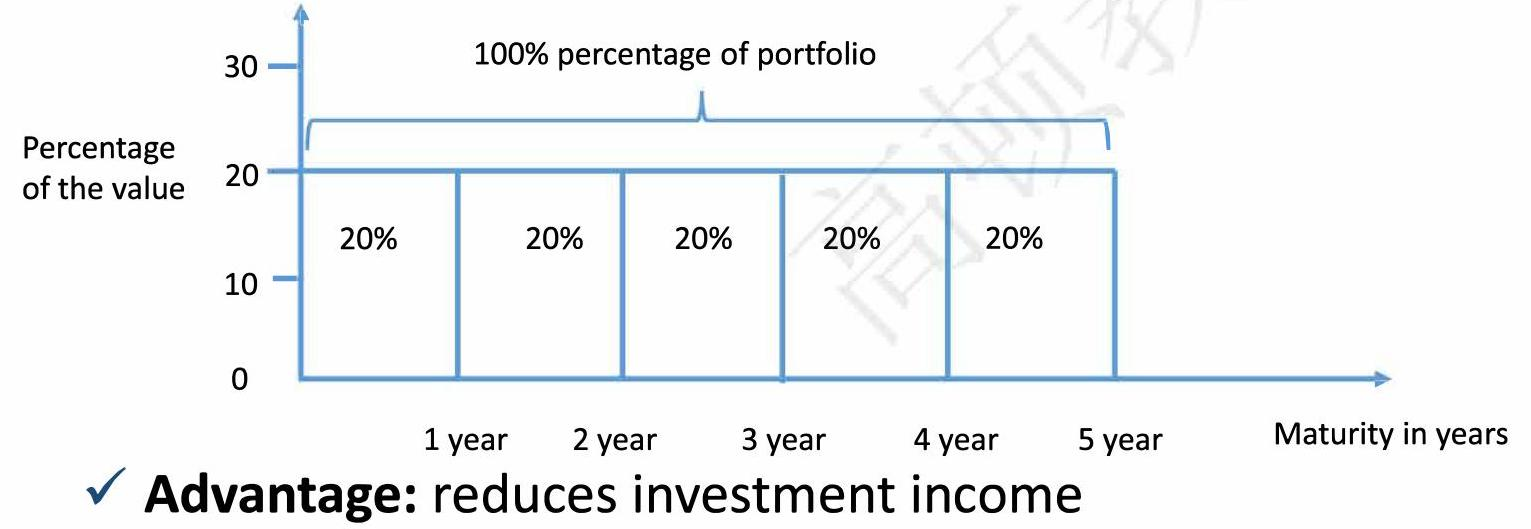
\includegraphics[width=0.5\textwidth]{images/ladder.jpg}
    \caption{ladder}
    \label{fig:labe19}
    \end{figure}
    \item Advantage: reduces investment income fluctuation/require little management expertise.
    \end{itemize}
\item The front-end load maturity policy
    \begin{itemize}
    \item Strategy: all security investments are short-term.
        \begin{figure}[H]
        \centering
        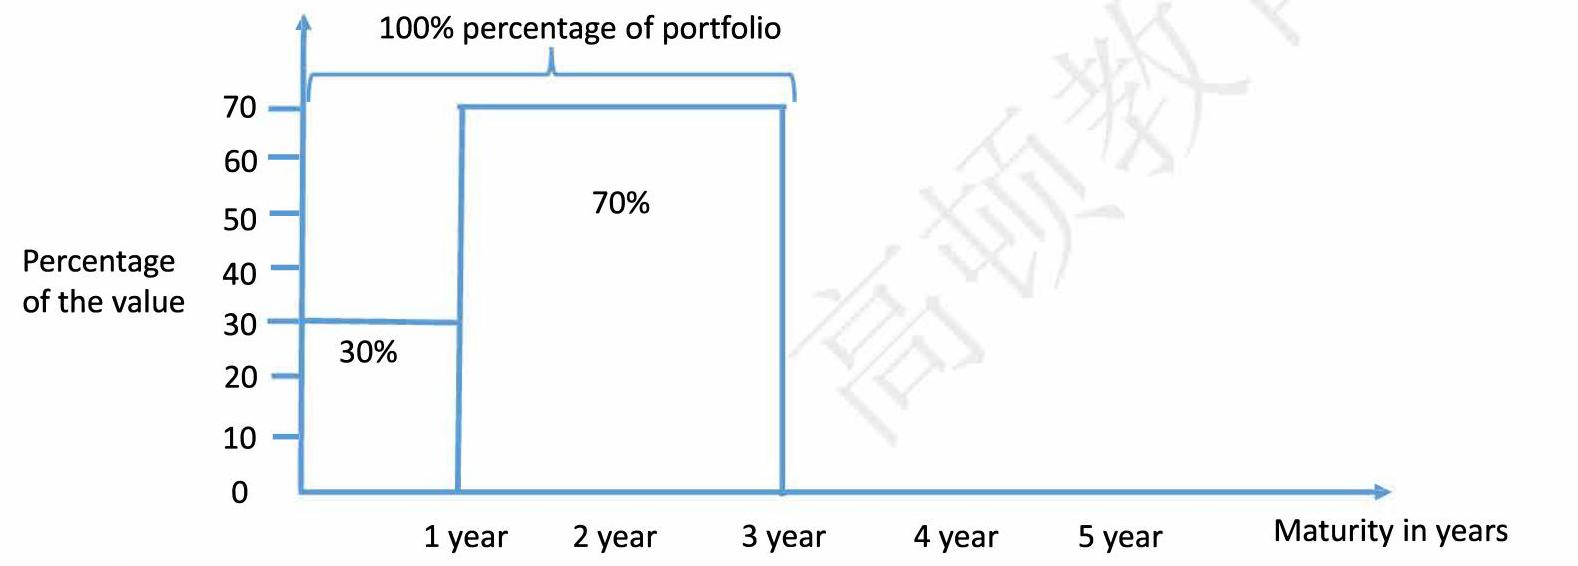
\includegraphics[width=0.5\textwidth]{images/front.jpg}
        \caption{front}
        \label{fig:labe20}
        \end{figure}
    \item Advantage: strengthens the financial firm's liquidity position and avoids large capital losses if market interest rate rise.
    \end{itemize}
\item The back-end load maturity policy
    \begin{itemize}
    \item Strategy: all security investments are long-term.
    \begin{figure}[H]
        \centering
        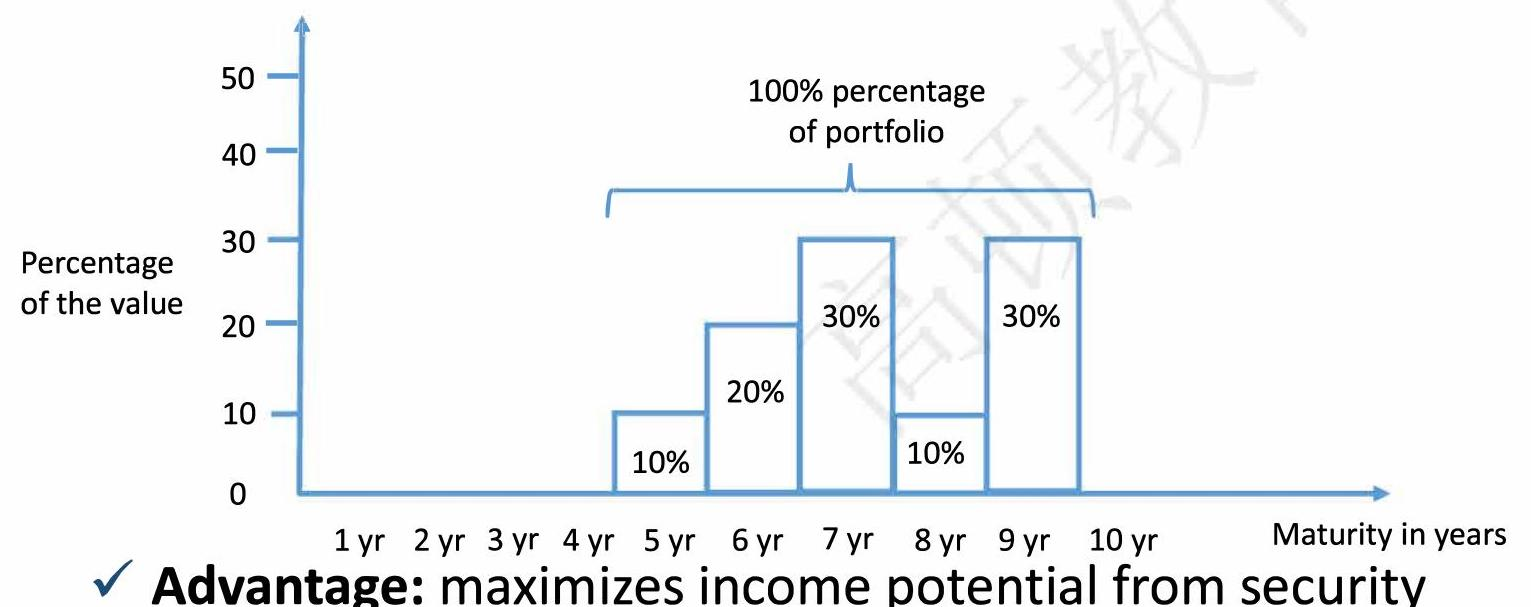
\includegraphics[width=0.5\textwidth]{images/back.jpg}
        \caption{back}
        \label{fig:labe21}
        \end{figure}
    \item Advantage: maximizes income potential from security investments if market interest rate fall.
    \end{itemize}
\item The barbell investment portfolio strategy
    \begin{itemize}
    \item Strategy: security holdings are divided between short-term and long-term.
        \begin{figure}[H]
        \centering
        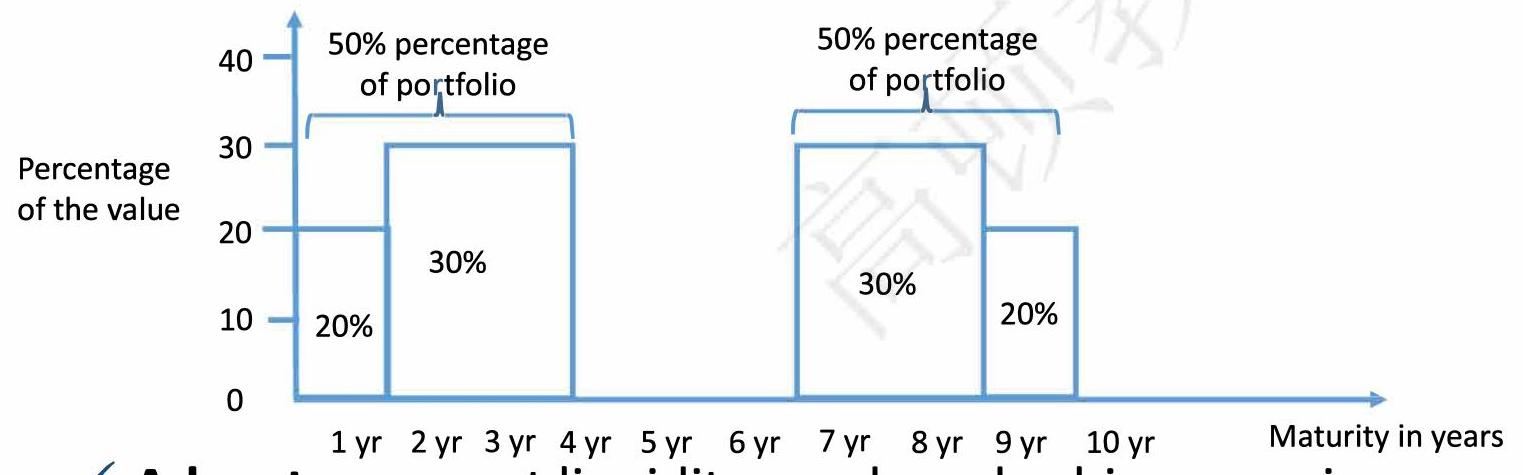
\includegraphics[width=0.5\textwidth]{images/barbell.jpg}
        \caption{barbell}
        \label{fig:labe22}
        \end{figure}
    \item Advantage: meet liquidity needs and achieve earnings goals.
    \end{itemize}
\item The rate-expectations approach
    \begin{itemize}
    \item Strategy: change the mix of investment maturities as the interest rate outlook changes.
        \begin{figure}[H]
        \centering
        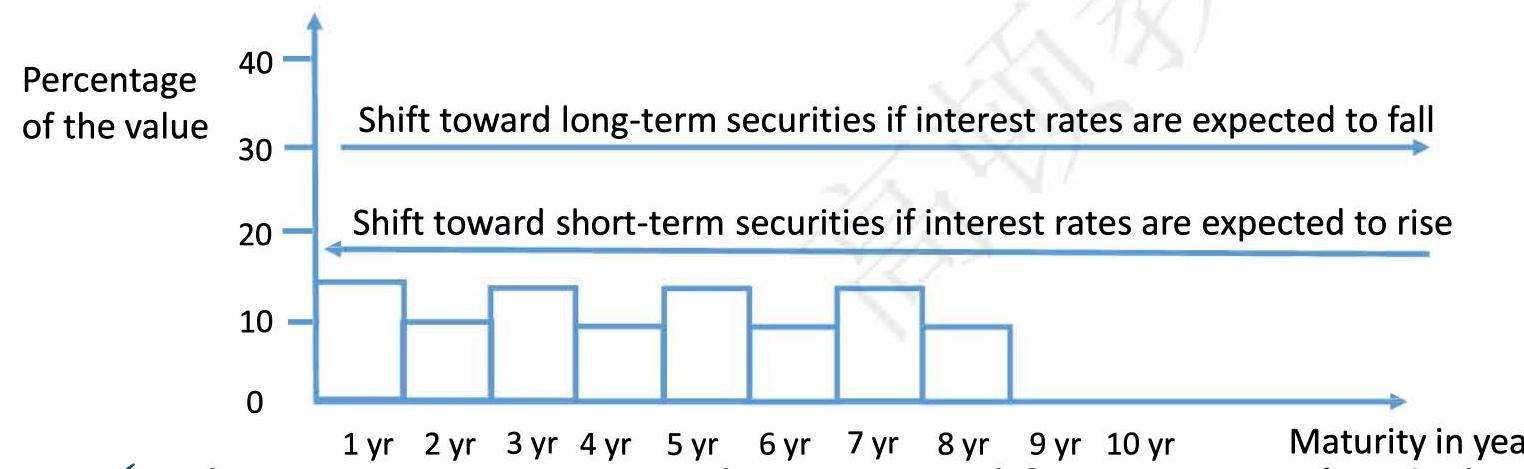
\includegraphics[width=0.5\textwidth]{images/rate.jpg}
        \caption{rate}
        \label{fig:labe23}
        \end{figure}
    \item Advantage: maximizes the potential for earnings (and also for losses).
    \end{itemize}
\end{itemize}



\subsubsection{Maturity management tools}
\begin{itemize}
\item The yield curve: a picture of how market interest rates differ across loans and securities of varying term (time) to maturity.
    \begin{itemize}
    \item Forecast interest rates and the economy
    \item Show current trade-offs between returns and risks
    \item Measure how much might be earned currently by pursuing the carry trade
    \item Riding the yield curve strategy: when the yield curve's slope is steep enough, buy the longer-term security (higher YTM) and hold until its tenor decreases (lower YTM), then sell it.
    \end{itemize}
    
\item Duration: present-value-weighted measure of maturity of an individual security or portfolio of securities.
    \begin{itemize}
    \item Immunization of interest rate risk and reinvestment risk offset each other:
        \begin{itemize}
        \item  Duration of an individual security or a security portfolio is set equal to the investing institution's planned holding period.
        \end{itemize}
        
   
    \end{itemize}
    
\end{itemize}



\subsubsection{Major lines of business of dealer banks}
\begin{itemize}
\item Intermediate in Securities dealing, underwriting, and trading
    \begin{itemize}
    \item Dealer的基础业务: Intermediate in the primary market between issuers and investors of securities and in the secondary market among investors
    \item Risk factors:
        \begin{itemize}
        \item short-term funding like repo
        \end{itemize}
    \end{itemize}
    
\item Trade in over-the-counter derivatives
    \begin{itemize}
    \item For most over-the-counter derivatives trades, one of the two counterparties is a dealer.
        \begin{itemize}
        \item Running matched book: aim to lay off much or all the risk of its positions by offset trades and made profits from the differences between bid and offer terms.
        \end{itemize}
    \item Proprietary trading in over-the-counter derivatives markets
    \item Risk factors:
        \begin{itemize}
        \item Contingent payments risk \& Counterparty risk
        \end{itemize}
    \end{itemize}
    
\item As Prime brokerage to hedge funds and other large investors
    \begin{itemize}
    \item 主经纪商业务：Provides services including management of securities holdings, clearing, cash-management services, securities lending, financing, and reporting
    \item 盈利方式: Generates additional revenues by lending securities that are placed by prime-brokerage clients
    \end{itemize}
    
\item Dealer banks have large asset-management divisions
    \begin{itemize}
    \item Cater to the investment needs of institutional and wealthy individual clients.
    \end{itemize}
    
\item Prime brokerage and asset management
    \begin{itemize}
    \item Risk factors: The dealer bank's liquidity position is weakened if large clients exit their positions or enter new positions to offset their risk
        \begin{itemize}
        \item Systemic liquidity crisis
        \end{itemize}
        
    \end{itemize}
    
\end{itemize}



\subsubsection{Failure mechanisms}
\begin{itemize}
\item "Run-on-the-bank": The key mechanisms that lead to the failure of a dealer bank:
    \begin{itemize}
    \item The flight of short-term creditors
    \item The departures of prime-brokerage clients
    \item Cash-draining actions by derivatives counterparties
    \item Loss of clearing-bank privileges
    \end{itemize}
\item The flight of short-term creditors
    \begin{itemize}
    \item Dealer bank 融资来源:
        \begin{itemize}
        \item Bonds and commercial paper
        \item  Short-term repos
        \end{itemize}
    \item During financial crisis, repo rollover becomes difficult.
        \begin{itemize}
        \item The dealer may be forced to sell its assets in a hurry, resulting in much lower prices. Lower price leads to further fire sales for others, causing a systemic risk.
        \end{itemize}
    \end{itemize}
\item The way to mitigate the risk of flight of short-term creditors:
    \begin{itemize}
    \item Establishing lines of bank credit
    \item Dedicating a buffer stock of cash and liquid securities for emergency liquidity needs
    \item "Laddering" the maturities of its liabilities so that only a small fraction of its debt must be refinanced within a short period of time.
    \end{itemize}
\item The departures of prime-brokerage clients
    \begin{itemize}
    \item Clients' balances: The prime broker can use clients' cash balances to meet the immediate cash demands of another.
    \item Rehypothecation: Margin loans for a dealer bank can also be financed using the client's own assets as collateral, through "rehypothecation."
    \item Clients' departures: If clients do leave without notice, their cash and securities are not in the pool, forcing dealer banks to use its own cash to meet liquidity needs.
    \end{itemize}
\item Cash-draining actions by derivatives counterparties
    \begin{itemize}
    \item If a dealer bank is in a solvency crisis, OTC counterparty would look for opportunities to reduce exposure to that dealer bank.
        \begin{itemize}
        \item Borrow from the dealer
        \item Enter new trades that cause dealer to pay out cash
        \item Seek to harvest cash from any derivatives positions
        \end{itemize}
    \item The way to mitigate the risk:
        \begin{itemize}
        \item Central clearing counterparty
        \end{itemize}
    \end{itemize}
\item Loss of cash settlement privileges
    \begin{itemize}
    \item Daylight overdraft privileges: Under normal conditions, clearing bank extend "daylight overdraft privileges" to creditworthy clearing customers.
    \item Refuse the privileges: The clearing bank may refuse to process transactions that are insufficiently funded by the dealer bank's cash fund account when the solvency of a dealer bank is questioned.
    \end{itemize}
\end{itemize}



\subsubsection{Policy responses to alleviate dealer's risk}
\begin{itemize}
\item Capital injections: central banks and by capital injections into dealer banks.
    \begin{itemize}
    \item Most important source of sy stemic risk is the potential impact of dealer-bank fire sales on market prices and investor portfolios.
    \end{itemize}
\item Higher capital requirements: capital are likely to be higher for derivatives that are not guaranteed by a central clearing counterparty.
\item Central-bank insurance for tri-party repos: Short-term triparty repos are a particularly unstable source of financing in the face of concerns over a dealer's solvency.
\item Central clearing: Threat by flight of OTC derivatives counterparties can be lowered by central clearing.
\item Pre-failure resolution: such as distress-contingent convertible debt of dealer banks are important for those are suffering grievous financial distress.
\end{itemize}



\subsection{Managing Deposit Services and Non-deposit Liabilities Ch12\& 13}



\subsubsection{Deposit Services}
\begin{itemize}
\item Deposit accounts are the number one source of funds at most banks. Two key issues:
    \begin{itemize}
    \item Where can funds be raised at lowest possible cost?
    \item How can management ensure that the institution always has enough deposits to support lending and other services the public demands?
    \end{itemize}
    
\end{itemize}



\subsubsection{Deposit types}
\begin{itemize}
\item Main type of deposit services types:
    \begin{itemize}
    \item Transaction (payment or demand) deposits: honor any withdrawals made by the customer immediately.
    \item Non-transaction (savings or thrift) deposits: Design to attract funds from customers who wish to set aside money for future expenditures or financial emergencies.
    \end{itemize}
\end{itemize}



\subsubsection{Transaction deposits}
\begin{itemize}
\item Noninterest-bearing transaction (demand) deposits
    \begin{itemize}
    \item Do not earn explicit interest but provide the customer with payment service.
    \item Most volatile and least predictable, and with shortest potential maturity.
    \end{itemize}
\item Interest-bearing transaction deposits
    \begin{itemize}
    \item Provide all the foregoing services and pay at least some interest.
    \item Negotiable order of withdrawal (NOW) accounts
        \begin{itemize}
        \item Hybrid checking-savings deposits
        \item Give the offering depository institution prior notice before the customer withdraws funds
        \item Held only by individuals and nonprofit institutions
        \end{itemize}
    \item Money market deposit accounts (MMDAs)
        \begin{itemize}
        \item Flexible money market interest rates but accessible via check or preauthorized draft to pay for goods and services.
            \begin{itemize}
            \item Up to six preauthorized drafts and three withdrawals be made by writing checks per month.
            \end{itemize}
        \item Can be held by businesses as well as individuals.
        \end{itemize}
    \item Super NOWs
        \begin{itemize}
        \item No limitation on the number of checks depositor write.
        \item Offers institutions post lower yields on SNOWs than on MMDAs.
        \item Can be held by individuals and nonprofit institutions.
        \end{itemize}
    \item Mobile apps
        \begin{itemize}
        \item The hottest item in the transaction deposit field today appears to be the mobile check deposit.
        \end{itemize}
    \end{itemize}
\item 
\end{itemize}



\subsubsection{Non-transaction deposits}
\begin{itemize}
\item Passbook saving deposits
    \begin{itemize}
    \item Unlimited withdrawal privileges and low interest rate
    \item Tend to be stable with little sensitivity to changes in interest rates.
    \item Individuals, nonprofit organizations, governments, and business firms can hold savings deposits
        \begin{itemize}
        \item Businesses could not place more than \$150,000 in the United States
        \end{itemize}
    \end{itemize}
\item Time deposits
    \begin{itemize}
    \item Provide to wealthier depositors with fixed maturity dates and fixed or sometimes fluctuating rates.
    \item Must carry a minimum maturity of 7 days.
    \item Most popular of all time deposits is certificates of deposits (CDs)
        \begin{itemize}
        \item Negotiable CD and nonnegotiable CD.
        \end{itemize}
    \end{itemize}
\item Retirement savings deposits
    \begin{itemize}
    \item Wage earners and salaried individuals: individual retirement account （IRA） grant the right to make limited tax-free contributions each year.
    \item Self-employed persons: Keogh plan retirement account is available.
    \item Both IRAs and Keoghs are highly stable and carries fixed interest rate, which are great appeal for managers of depository institutions.
    \end{itemize}
\end{itemize}


\begin{figure}[H]
    \centering
    \begin{tikzpicture}[
      node distance=1.7cm and 2.2cm,
      every node/.style={draw, rounded corners, align=center, font=\small, minimum width=2.8cm, minimum height=0.9cm},
      edge from parent/.style={draw, -latex}
      ]
    % 一级
    \node (deposit) {deposit};
    % 二级
    \node (td) [right=of deposit, yshift=1.5cm] {Transaction\\ deposits};
    \node (ntd) [right=of deposit, yshift=-1.5cm] {Non-transaction\\ deposits};
    % 三级
    \node (nibtd) [right=of td, yshift=1.2cm] {Noninterest-\\bearing transaction\\ deposits};
    \node (ibtd) [right=of td, yshift=-0.2cm] {Interest-bearing\\ transaction deposits};
    \node (ma) [right=of td, yshift=-1.6cm] {Mobile apps};
    \node (psd) [right=of ntd, yshift=0.7cm] {Passbook saving\\ deposits};
    \node (td2) [right=of ntd, yshift=-0.7cm] {Time deposits};
    \node (rsd) [right=of ntd, yshift=-2.1cm] {Retirement\\ savings deposits};
    % 四级
    \node (now) [right=of ibtd, yshift=1.2cm] {Negotiable order of\\ withdrawal (NOW)\\ accounts};
    \node (mmda) [right=of ibtd, yshift=0cm] {Money market deposit\\ accounts (MMDAs)};
    \node (snow) [right=of ibtd, yshift=-1.2cm] {Super NOWs};
    
    % 连线
    \draw[->] (deposit) -- (td);
    \draw[->] (deposit) -- (ntd);
    
    \draw[->] (td) -- (nibtd);
    \draw[->] (td) -- (ibtd);
    \draw[->] (td) -- (ma);
    
    \draw[->] (ntd) -- (psd);
    \draw[->] (ntd) -- (td2);
    \draw[->] (ntd) -- (rsd);
    
    \draw[->] (ibtd) -- (now);
    \draw[->] (ibtd) -- (mmda);
    \draw[->] (ibtd) -- (snow);
    
    \end{tikzpicture}
    \caption{存款类型结构图}
    \end{figure}

\subsubsection{Pricing Deposits}
\begin{itemize}
\item An important issue remains: How should depository institutions price their deposit and deposit services in order to attract new funds and make a profit?
    \begin{itemize}
    \item Need to pay a high enough interest return to attract customer funds but must avoid paying an interest rate so costly that it erodes any potential profit margin.
    \end{itemize}
\end{itemize}



\subsubsection{Deposits and Deposit Services Pricing Methods}
\begin{itemize}
\item Marginal Cost
\item Cost plus profit margin
\item Conditional Pricing
\item Relationship pricing
\end{itemize}



\subsubsection{Deposits Pricing Methods}
\begin{itemize}
\item Marginal Cost
    \begin{itemize}
    \item Definition: the added cost of bringing in new funds.
    \item Formular: Marginal cost rate = $\dfrac{Change in total cost}{Addictional funds raised}$
        \begin{itemize}
        \item Change in total cost (Marginal cost)= New interest rate × Total funds raised at new rate - Old interest rate × Total funds raised at old rate
        \end{itemize}
    \item Profit maximum
        \begin{itemize}
        \item  marginal revenue rate = marginal cost rate
        \end{itemize}
    \end{itemize}
\item Example

    \begin{itemize}
    \item New Day Bank plans to launch a new deposit campaign next week in hopes of bringing in from \$100 million to \$600 million new deposit, which it expects to invest at a 4.05 percent yield. The following chart is the cost for attracting new deposits.
    
    \begin {tabular}{|l|l|l|l|l|l|l|}
\hline
New Deposits (in millions) & 100 & 200 & 300 & 400 & 500 & 600 \\ \hline
Interest cost & 2\% & 2.25\% & 2.5\% & 2.75\% & 3\% & 3.25\% \\ \hline
\end {tabular}
    \item What interest rate should the institution set to ensure that profit is maximized?
    \item Answer:
    
    \begin{tabular}{|p{2.5cm}|p{2.5cm}|p{2.5cm}|p{2.5cm}|p{2.5cm}|p{2.5cm}|}
        \hline
        Expected Amounts of New Deposits That Will Flow In & Average Interest the Bank Will Pay on New Funds & Total Interest Cost of New Funds Raised & Marginal Cost of New Deposit Money & Marginal Costs as a Percentage of New Funds & Total Profits Earned (after interest cost) \\ \hline
        100 & 2\% & 2 & 2 & 2\% & 2.05 \\ \hline
        200 & 2.25\% & 4.5 & 2.5 & 2.5\% & 3.60 \\ \hline
        300 & 2.5\% & 7.5 & 3 & 3\% & 4.65 \\ \hline
        400 & 2.75\% & 11 & 3.5 & 3.5\% & 5.20 \\ \hline
        \color{blue}500 & \color{blue}3\% & \color{blue}15 & \color{blue}4 & \color{blue}4\% & \color{blue}5.25 \\ \hline
        600 & 3.25\% & 19.5 & 4.5 & 4.5\% & 4.80 \\ \hline
\end{tabular}


    \item The institution should set deposit interest rate at 3\%
    \end{itemize}
\end{itemize}



\subsubsection{Deposit Services Pricing Methods}
\begin{itemize}
\item Cost plus profit margin
    \begin{itemize}
    \item Each deposit service may be priced high enough to recover all or most of the cost of providing that service.
    \item Calculate formula:
    \begin{align*}
        \text{Unit price charged the customer for each deposit service} &= \text{Operating expense per unit of deposit service} \nonumber \\
        &+ \text{Estimated overhead expense allocated to deposit service} \nonumber \\
        &+ \text{Planned profit margin from each service unit sold}
        \end{align*}
    \end{itemize}
\item Example
    \begin{itemize}
    \item G\&F Savings Bank finds that its basic transaction account, which requires a \$1000 minimum balance, costs an average of \$3.25 per month in servicing costs (including labor and computer expense) and \$1.25 per month in overhead expenses. The bank also tries to gain a \$0.50 per month profit margin on these accounts. What monthly fee should the bank charge each customer?
    \item Answer:
        \begin{itemize}
        \item \$3.25 + \$1.25 + \$0.50 = \$ 5
        \end{itemize}
    \end{itemize}
\item Conditional Pricing
    \begin{itemize}
    \item The customer pays a low fee or no fee if the deposit balance remains above some minimum level but faces a higher fee otherwise.
    \item Varies among deposits based on one or more factors as follows:
        \begin{itemize}
        \item The number of transactions
        \item The average balance
        \item The maturity of the deposit
        \end{itemize}
    \item Flat-rate pricing
        \begin{itemize}
        \item The depositor's cost is a fixed charge per check, per time period, or both.
        \end{itemize}
    \item Free pricing
        \begin{itemize}
        \item No monthly account maintenance fee or per-transaction charge.
        \item Unprofitable for institutions because it tends to attract many small, active deposits when market rate is high.
        \end{itemize}
    \item Conditionally free pricing
        \begin{itemize}
        \item Favors large-denomination deposits because services are free if the account balance stays above some minimum figure.
        \end{itemize}
    \end{itemize}
\item Relationship pricing
    \begin{itemize}
    \item Promotes greater customer loyalty
    \item makes the customer less sensitive to the prices posted on services offered by competing financial firms.
    \end{itemize}

    \begin{figure}[H]
        \centering
        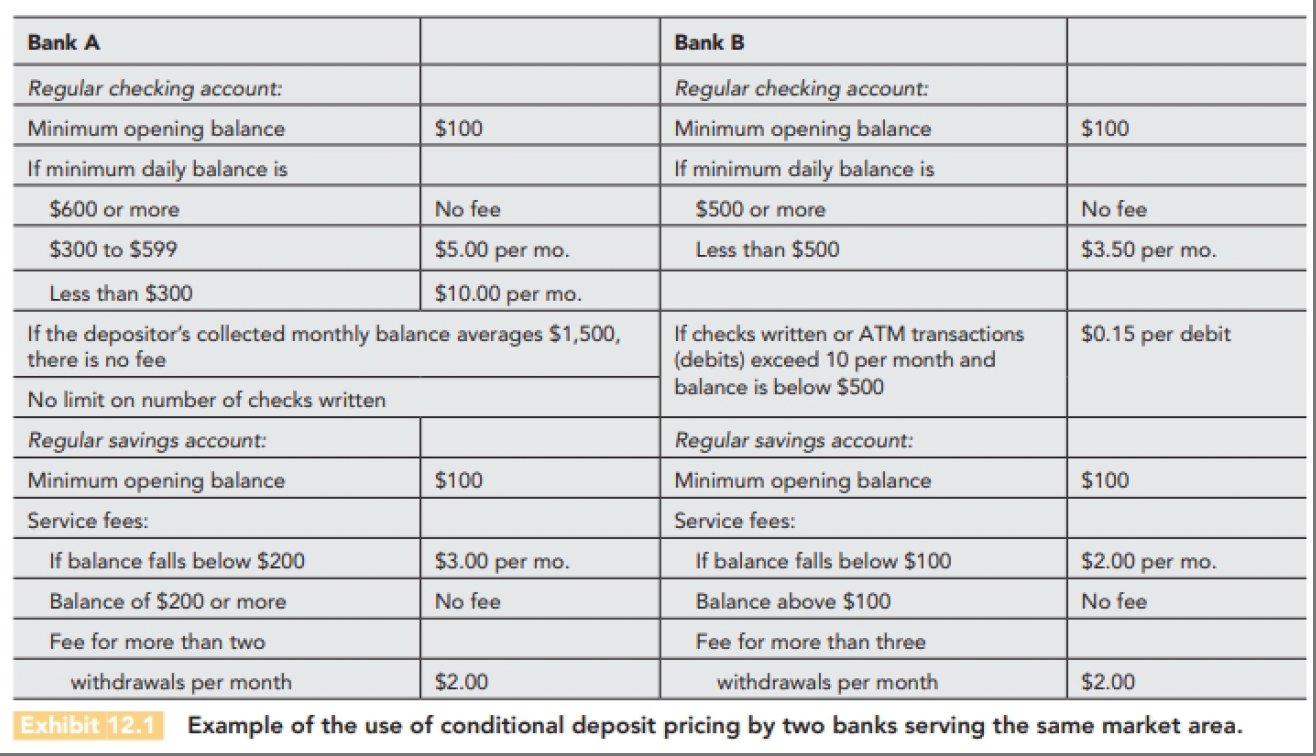
\includegraphics[width=1\textwidth]{images/DEPOSITPRICE.png}
        \caption{DEPOSITPRICE}
        \label{fig:labe21}
        \end{figure}
    
\item Deposit insurance
    \begin{itemize}
    \item 供保机构: Federal Deposit Insurance Corporation (FDIC) provides deposit protection for its membership.
    \item 免责范围: U.S. government securities, shares in mutual funds, safe deposit boxes, and funds stolen from an insured depository institution.
    \item 保费制定: determined by the volume of deposits and the degree of risk exposure.
    \end{itemize}
\item Disclosure of deposit service
    \begin{itemize}
    \item Advertising of deposit terms may not be misleading.
    \item Deposit rates must be quoted as annual percentage yields(APY).
    \item The dates and minimum balance required must be explicit.
    \item The depositor must be warned of penalties or fees that could reduce the yield.
    \end{itemize}

\end{itemize}



\subsubsection{Overdraft protection}
\begin{itemize}
\item Definition: This service makes sure that clients' incoming checks and draft are paid and clients avoid excessive NSF (not sufficient funds) fees.
    \begin{itemize}
    \item Provide customers convenience but like predatory lending
    \item High actual interest rate: Important source of income for financial-service provider.
    \end{itemize}
\item Being criticized: Faced with adverse public and regulators' comments, some financial firms have reduced or eliminated their overdraft fees.
\end{itemize}



\subsubsection{Basic (Lifeline) Banking}
\begin{itemize}
\item Controversial social issue: Depository institutions are asked to offer low-cost financial services, especially deposits and loans, for customers unable to afford conventional services.
    \begin{itemize}
    \item Controversial for service provider:
        \begin{itemize}
        \item Low price cannot cover cost: Most financial-service providers are privately owned corporations and responsible to their shareholders to earn profit.
        \item Regulation problem: banking industry is regulated and are not treated in public policy like other private firms.
        \end{itemize}
    \item Controversial for solving the issue:
        \begin{itemize}
        \item How to decide which customers access to low-price
        services?
        \item Insist on imposing a means test on customer?
        \item Someone must bear the cost of producing services but
        who?
        \end{itemize}
    \end{itemize}
    
\end{itemize}



\subsubsection{Practices}
\begin{itemize}
\item First Metrocentric Bank posts the following schedule of fees for its household and small-business transaction accounts: For average monthly account balances over \$1,500, there is no monthly maintenance fee and no charge per check or other draft. For average monthly account balances of \$1,000 to \$1,500, a \$2 monthly maintenance fee is assessed and there is a \$1 charge per check or charge cleared. For average monthly account balances of less than \$1,000, a \$4 monthly maintenance fee is assessed and there is a \$1.5 per check or per charge fee. What form of deposit pricing is this?

A. Cost plus profit margin

B. Marginal Cost

C. Conditional Pricing

D. Relationship pricing

\item Answer: C

解析:根据题目描述，可以得知不同的存款余额的条件下，对于账户的收费是不一样的，属于条件定价。
\end{itemize}



\subsubsection{Sources of Non-deposit Liabilities}
\begin{itemize}
\item When deposit is inadequate to support loans and investment, financial institutions need non-deposit liabilities:
    \begin{itemize}
    \item Federal Funds Market (Most popular domestic source)
    \item Borrowing from Federal Reserve Banks
    \item Advances from Federal Home Loan Banks
    \item The large Negotiable CDs
    \item The Eurocurrency Deposit Market
    \item Commercial Paper market
    \item Repurchase Agreements
    \item Long-term non-deposit funds
    \end{itemize}
    
\item Federal Funds Market ("Fed Funds"): Consist exclusively of deposits held at the Federal Reserve banks and can be transferred through Fedwire.
    \begin{itemize}
    \item Meet legal reserve requirements and satisfy loan demand
    \item Large banks play a role similar to funds brokers.
    \item Short-term borrowings:
        \begin{itemize}
        \item Overnight loans: Normally no collateral
        \item Term loans: longer-term Fed loans contract
        \item Continuing contract: automatically renewed each day
        \end{itemize}
    \end{itemize}
    
\item Borrowing from Federal Reserve Banks: Fed will make the loan through its discount window by crediting the borrower's reserve account. The loan must be backed by acceptable collaterals.
    \begin{itemize}
    \item Primary credit: short terms(overnight to 90 days), a higher interest rate than Fed funds interest rate.
    \item Secondary credit: depository institutions not qualifying for primary credit, a higher interest rate than primary credit.
    \item Seasonal credit: longer periods than primary credit, for small and medium-sized institutions experiencing seasonal swings.
    \end{itemize}
    
\item Advances from Federal Home Loan Banks (FHLB)
    \begin{itemize}
    \item 目标: Improves the liquidity of home mortgages and encourages more lenders to provide credit to the housing market.
    \item 提供纾困抵押贷款: Allows troubled institutions to use the home mortgages as collateral for emergency loans.
    \item 贷款利率低于市场利率: A stable source of funding at below-market interest rates.
    \item 期限范围广: Ranges from overnight to more than 20 years
    \end{itemize}
    
\item The large Negotiable CDs
    \begin{itemize}
    \item A hybrid account: a deposit or another form of IOU.
    \item  Short maturity: range from 7 days to 1 or 2 years but concentrated in the 1- to 6-month.
    \item 到期本息和的计算：Amount due CDs = Principal + Principal $\times\dfrac{Days\ to\ maturity}{360\ days}\times$ Annual interest rate
    \end{itemize}
    
\item The Eurocurrency Deposit Market
    \begin{itemize}
    \item How to borrow and lend Eurocurrencies: A domestic financial firm can tap the Euromarkets for funds by contacting one of the major international banks that borrow and lend Eurocurrencies every day.
        \begin{itemize}
        \item The largest U.S. bank use their own overseas branches tap the market.
        \end{itemize}
    \item The largest unregulated financial market-place in the world.
    \end{itemize}
    
\item Commercial Paper market
    \begin{itemize}
    \item Short-term notes: 3 or 4 days to 9 months, sell at discount.
    \item Industrial paper: designed to finance the purchase of inventories or raw materials and to meet other immediate cash needs of nonfinancial companies.
    \item Financial paper: issued by finance companies and the affiliates of financial holding companies.

        \begin{itemize}
        \item  Purchase off-book loans of other financial firms in same organization, giving these firms funds to make new loans.
        \end{itemize}
    \end{itemize}
   
    
\item Repurchase Agreements
    \begin{itemize}
    \item Less popular than Fed funds and more complex.
    \item Most domestic Repos are transacted across the Fed Wire system, just as are Fed funds transactions.
    \item A bit longer time to transact than a Fed funds loan.
    \item Repo transaction is often for overnight funds, but it may be extended for days, weeks, or even months.
    \end{itemize}
    
\item Long-term non-deposit funds
    \begin{itemize}
    \item Beyond one year: 5 to 12 years mortgages, capital notes and debentures.
    \item Favorable leveraging effect: made it attractive to larger financial firms.
    \item More sensitive: Tend to be a sensitive barometer of the perceived risk exposure.
    \end{itemize}
    
\item 
\end{itemize}



\subsubsection{Non-deposit Funding Choice}
\begin{itemize}
\item In using non-deposit funds, funds managers must answer the following key questions:
    \begin{itemize}
    \item 1. How much in total must be borrowed from these sources to meet funding needs?
    
    • Available Funds Gap
    \item 2. Which non-deposit sources are best, given the borrowing institution's goals?
    
    • The relative costs, risk, length of time, size of the institution, regulations limits.
    \end{itemize}
\end{itemize}



\subsubsection{Available Funds Gap (AFG)}
\begin{itemize}
\item Calculation formular:
    \begin{itemize}
    \item \begin{align*}
        \text{Available funds gap (AF)}&=\text{Current and projected loans and investments the}\\
        &\quad\text{lending institution desires to make}\\
        &-\text{Current and expected deposit inflows and other}\\
        &\quad\text{available funds}
        \end{align*}
    \item Small amount add to AFG: cover unexpected credit demands or unanticipated shortfalls in inflow funds.
    \end{itemize}
\item Example
    \begin{itemize}
    \item Suppose a commercial bank has new loan request that meet its quality standards for \$150 million, it wishes to purchase \$75 million in new Treasury securities and expects drawings on credit lines from its customers of \$135 million. Deposit and other customer funds received today total \$185 million, and those expected in the coming week will be \$100 million.
    \item Answer:
        \begin{itemize}
        \item AFG= (\$150 + \$75 + \$135) - (\$185 + \$100) = \$75m
        \end{itemize}
    \end{itemize}
\end{itemize}



\subsubsection{Factors of choosing alternative non-deposit sources}
\begin{itemize}
\item The relative costs of raising funds from each source.
\item The risk (volatility and dependability) of each funding source.
\item The length of time (maturity or term) for which funds are needed.
\item The size of the institution that requires funds.
\item Regulations limiting the use of alternative funds sources.
\item The relative costs of raising funds
    \begin{itemize}
    \item Effective cost rate: determine how much each source of borrowed funds costs.
    \end{itemize}
\item The relative costs of raising funds from each source
\begin{align*}
        \text{Effective cost rate on funds} &= \frac{\text{(Current interest cost on amounts borrowed+ Noninterest costs incurred to access these funds)}} {\text{Net investable funds raised from this source}}
        \end{align*}
 \begin{align*}
            \text{Current interest cost on amounts borrowed} &= \text{Prevailing interest rate in the money market} \quad \times \text{Amount of funds borrowed}
            \end{align*}
    \begin{itemize}
    \item Noninterest costs to access funds = (Estimated cost rate representing staff time, facilities, and transaction costs) x Amount of funds borrowed
    \item Net investable funds = Total amount borrowed less legal reserve requirements (if any), deposit insurance (if any), and funds placed in nonearning assets
    \item Deposit insurance = Total deposits received from the public x Insurance fee per dollar
    \end{itemize}
\item Example: Effective cost rate
    \begin{itemize}
    \item Suppose that Fed funds are currently trading at an interest rate of 6.0 percent. Moreover, management estimates that the marginal noninterest cost, in the form of personnel expenses and transactions fees, from raising additional monies in the Fed funds market is 0.25 percent. Suppose that a depository institution will need \$25 million to fund the loans it plans to make today, of which only \$24 million can be fully invested due to other immediate cash demands. What is the effective cost rate Fed funds ?
    \item Answer
    
    Current interest cost on Federal funds = 0.06 x \$25m = \$1.5m

    
Noninterest cost to access Federal funds raised = 0.0025 x \$25m = \$0.063m

\begin{align*}
    \text{The effective annualized Fed funds cost rate} &= \frac{\$1.5\ \text{m} + \$0.063\ \text{m}}{\$24\ \text{m}} \\
    &= 6.51\%
    \end{align*}
    \end{itemize}

\item Example: Effective cost rate considering insurance fee
    \begin{itemize}
    \item Suppose management decides to consider borrowing funds by issuing negotiable CDs that carry a current interest rate of 7.00 percent. Moreover, raising CD money costs 0.75 percent in noninterest costs. An additional expense associated with selling CDs to raise money is the deposit insurance fee, assume the current insurance rate is \$0.0027 per dollar of deposits. What is the effective cost rate of negotiable CDs?
    \item Answer
    \begin{align*}
        \text{Current interest cost on negotiable CDs} &= 0.07\times\$25\text{m} = \$1.75\text{m}\\
        \text{Noninterest cost to negotiable CDs} &= 0.0075\times\$25\text{m} = \$0.1875\text{m}\\
        \text{Insurance fee} &= \$25\ \text{million}\times0.0027 = 0.0675\text{m}\\
        \text{Effective cost rate} &= \frac{(1.75\text{m}+0.1875\text{m})}{\$24\ \text{million}-\$0.0675\ \text{million}} = 8.10\%
        \end{align*}
    \end{itemize}

\item The risk (Volatility and dependability) of each funding source.
    \begin{itemize}
    \item Interest rate risk: The volatility of credit costs, the shorter the term of the loan, the more volatile the prevailing market interest rate tends to be.
    \item Credit availability risk: Negotiable CD, Eurodollar, and commercial paper markets are especially sensitive to credit availability risks.
    \end{itemize}
\item The length of time (maturity and term) funds are needed
    \begin{itemize}
    \item Some funds sources, such as commercial paper and longterm debt capital may be difficult to access immediately.
    \item Term or maturity of the funds need plays a key role as well.
    \end{itemize}
\item The size of the borrowing institution
    \begin{itemize}
    \item The standard trading unit for most money market loans is \$1 million.
    \item The Fed funds and central bank's discount window can make small denomination loans for smaller firms.
    \end{itemize}
\item Regulations limiting the use of alternative funds sources
    \begin{itemize}
    \item Federal and state regulations may limit the amount, frequency, and use of borrowed funds.
        \begin{itemize}
        \item In the United States CDs must be issued at least 7 days.
        \item The Federal Reserve banks may limit borrowings from the discount window, particularly by depository institutions that appear to display significant risk of failure.
        \item Other forms of borrowing may be subjected to legal reserve requirements by action of the central bank.
        \end{itemize}
        
    \end{itemize}
\item 


\end{itemize}



\subsubsection{Overall cost of funds calculation}
\begin{itemize}
\item The relative costs of raising funds from various sources including deposits
    \begin{itemize}
    \item Historical average cost approach (look at the past)    
        \begin{itemize}
        \item Weighted average interest expense
        \item Break-even cost (cover the operating and interest cost)
        \item Weighted average overall cost of capital
        \end{itemize}
    \item Pooled-funds approach (look at the future)
        \begin{itemize}
        \item Pooled deposit and nondeposit funds expense rate
        \item Hurdle rate
        \end{itemize}
    \item Example: Historical Average Cost Approach
        \begin{itemize}
        \item A bank needs to raise fund for future loans, it asks what funds the financial firm has raised to date and what they cost:
            \begin{table}[h]
            \centering
            \begin{tabular}{|l|c|c|}
            \hline
            Sources of Funds Drawn & Average Amount of Funds Raised (millions) & Average Rate of Interest Incurred \\ \hline
            Noninterest - bearing demand deposits & \$100 & 0\% \\ \hline
            Interest - bearing transaction deposits & \$200 & 7\% \\ \hline
            Savings accounts & \$100 & 5\% \\ \hline
            Time deposits & \$500 & 8\% \\ \hline
            Money market borrowing & \$100 & 6\% \\ \hline
            \end{tabular}
            \end{table}
        \item Assumed the operating costs is \$10 million and all earning assets is \$750 million, what is the weighted average interest expense and break-even cost rate on borrowed funds invested in earning assets? Assumed the required rate of return of \$100 million investment from stockholders is 12\% after tax (tax rate is 35\%), what is the weighted average overall cost of capital?
        \item Answer
        
        
\begin{table}[htbp]
    \centering
    \begin{tabular}{|>{\raggedright\arraybackslash}p{4.3cm}|
                    >{\centering\arraybackslash}p{2.5cm}|
                    >{\centering\arraybackslash}p{2.8cm}|
                    >{\centering\arraybackslash}p{3.2cm}|}
    \hline
    Sources of Funds Drawn Upon & 
    Avg. Amount (millions) & 
    Avg. Interest Rate & 
    Interest Paid (millions) \\
    \hline
    Noninterest-bearing demand deposits & \$100 & 0\% & \textcolor{red}{\$0} \\
    \hline
    Interest-bearing transaction deposits & \$200 & 7\% & \textcolor{red}{\$14} \\
    \hline
    Savings accounts & \$100 & 5\% & \textcolor{red}{\$5} \\
    \hline
    Time deposits & \$500 & 8\% & \textcolor{red}{\$40} \\
    \hline
    Money market borrowing & \$100 & 6\% & \textcolor{red}{\$6} \\
    \hline
    \multicolumn{2}{|c|}{{Total funds raised = \$1,000}} & \multicolumn{2}{c|}{{All interest costs = \$65}} \\
    \hline
    \end{tabular}


    \caption{Summary of Fund Sources and Associated Interest Costs}
    \end{table}

    \begin{align*}
        \text{Weighted average interest expense} &= \frac{\text{All interest paid}}{\text{Total funds raised}} = \frac{65}{1,000} = 6.5\% \\
        \text{break - even cost rate} &= \frac{\text{Interest} + \text{Other operating costs}}{\text{All earnings assets}} = \frac{65 + 10}{750} = 10\%
        \end{align*}
        \begin{align*}
            &\text{Weighted average overall cost of capital} \\
            =&\text{Break - even cost on borrowed funds} + 
            \frac{\text{After - tax cost of stockholders}'\text{investment}}{1 - \text{Tax rate}} \times \frac{\text{Stockholders}'\text{investment}}{\text{Earning assets}} \\
            =& 10\% + \frac{12\%}{1 - 0.35} \times \frac{100}{750} = 12.5\%
            \end{align*}
            \item Tips: 12.5\% is the lowest rate of return over all fund-raising costs and the borrowing institution can afford to earn on its assets if its equity shareholders invest \$100 million in the institution.
        \end{itemize}
    \item Example: Pooled-funds approach
        \begin{itemize}
        \item A bank needs to raise for future loans. Suppose the estimate for future funding sources and costs is as follows:
        
        \begin{table}[htbp]
    \centering
    \begin{tabular}{|>{\raggedright\arraybackslash}p{4.2cm}|
                    >{\centering\arraybackslash}p{3cm}|
                    >{\centering\arraybackslash}p{3.4cm}|
                    >{\centering\arraybackslash}p{3.2cm}|}
    \hline
    Profitable New Deposits and Nondeposit Borrowings &
    Dollars of New Deposit \& Borrowing (millions) &
    Portion Placed in New Earning Assets &
    Interest \& Other Operating Expenses \\
    \hline
    Interest-bearing transaction deposits & \$100 & 50\% & 8\% \\
    \hline
    Time deposits & \$100 & 60\% & 9\% \\
    \hline
    New stockholders’ investment & \$100 & 90\% & 13\% \\
    \hline
    \end{tabular}
    \caption{Summary of New Deposit and Investment Sources}
    \end{table}

    What is the Pooled deposit and non-deposit funds expense rate and what is the hurdle rate of return over all earning assets ?

    \item Answer

    \begin{table}[h]
        \centering
        \renewcommand{\arraystretch}{1.4}

        \begin{tabular}{|p{2.5cm}|p{2.5cm}|p{2.5cm}|p{2.5cm}|p{2.5cm}|p{2.5cm}|}
        \hline
        Profitable New Deposits and Nondeposit Borrowings & 
        Dollars of New Deposit \& Nondeposit Borrowing (millions) & 
        Portion of New Borrowings Placed in New Earning Assets & 
        Dollar Amount Placed in Earnings Assets (millions) & 
        Interest Expense \& Other Operating Expenses of Borrowing & 
        All Operating Expense Incurred (millions) \\ \hline
        Interest - bearing transaction deposits & \$100 & 50\% & \$50 = 100 × 50\% & 8\% & \$8 = 100 × 8\% \\ \hline
        Time deposits & \$100 & 60\% & \$60 = 100 × 60\% & 9\% & \$9 = 100 × 9\% \\ \hline
        New stockholders’ investment in the institution & \$100 & 90\% & \$90 = 100 × 90\% & 13\% & \$13 = 100 × 13\% \\ \hline
        Total & \$300 &  & \$200 &  & \$30 \\ \hline
        \end{tabular}
        \end{table}
    \begin{itemize}
        \item 
        \begin{align*}
            \text{Pooled deposit and nondeposit funds expense rate}
            =\frac{\text{All expected operating expenses}}{\text{All new funds expected}}=\frac{\$30}{\$300}=10\%
        \end{align*}
        \item 
        \begin{align*}
            \text{Hurdle rate of return over all earning assets} =\frac{\text{All expected operating expenses}}{\text{Dollars available to place in earnings assets}}=\frac{\$30}{\$200}=15\%
        \end{align*}
        \end{itemize}
        Tips: Hurdle rate of return over all earning assets: minimum rate of return must be earned on any future loans and investments just to cover the cost of all new funds raised.
        

        \end{itemize}
    \end{itemize}
    
\end{itemize}


\subsection{Repos And Financing Ch14}



\subsubsection{Repurchase Agreements Introduction}
\begin{itemize}
\item A contract in which a security is traded at some initial price with the understanding that the trade will be reversed at some future date at some fixed price.
    \begin{itemize}
    \item Repo rate: actual/360, simple rate
    \item Repo haircut: difference between the purchase price of the securities and the amount borrowed from the repo.
    \item Collateral: investors care about the quality of the collateral
    \item Margin call: borrower supplies extra collateral in declining markets but may withdraw collateral in advancing markets.
    \end{itemize}
    
\end{itemize}





\subsubsection{Repurchase Agreements calculation}
\begin{itemize}
\item Interest cost of Repo = Amount borrowed x Repo rate x Number of days in Repo borrowing /360 days
\item Amount borrowed(cash inflow) = collateral securities full price (invoice price) x (1 - haircut)
\item Cash outflow = Amount borrowed + Interest cost of Repo
\end{itemize}




\subsubsection{Example}
\begin{itemize}
\item Bank Venus buys a bond on its coupon payment date. Three months later, in order to generate immediate liquidity, the bank decides to repo the bond with Bank Lu. Details of the bond and repo transaction are in the following chart. If the repo contract expires 6 months (184 days) from now, what is the bank's expected cash outflow at the end of the repo transaction?

    \begin{table}[h]
    \centering
    \begin{tabular}{|l|l|}
    \hline
    Notional & (USD) 1000,000 \\ \hline
    Coupon (semi - annual) & 6\% \\ \hline
    Current quote bond price & (USD) 97.5 \\ \hline
    Repo haircut & 5\% \\ \hline
    Repo interest rate & 1.05\% \\ \hline
    \end{tabular}
    \end{table}
\item Answer
\begin{itemize}
    \item Cash inflow at beginning of repo:
    \begin{align*}
    1000000\times(97.5\% + 6\% \times 0.25)\times(1 - 5\%) = 940500
    \end{align*}
    \item Cash outflow at end of repo:
    \begin{align*}
    940500\times\left(1 + 1.05\% \times\frac{184}{360}\right) = 945547.35
    \end{align*}

\begin{figure}[H]
    \centering
    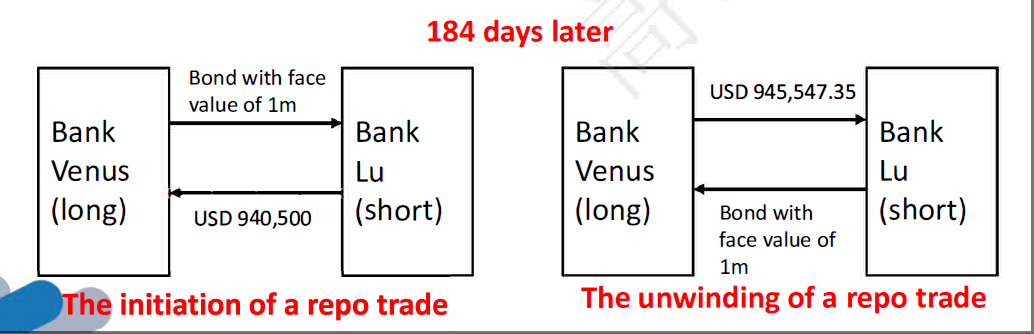
\includegraphics[width=0.5\textwidth]{images/iu.png}
    \caption{cash}
    \label{fig:labe18}
\end{figure}
\end{itemize}
\end{itemize}




\subsubsection{Common motivations for investing repo}
\begin{itemize}
\item Reverse Repos and Short Positions
    \begin{itemize}
    \item Buy the repo/ enter into reverse repo/ invest in repo: lender of cash in repo market
        \begin{itemize}
        \item Professional investors often want to short a bond.
            \begin{itemize}
            \item Bet the interest rates will rise
            \item Bet that the price of another security will rise relative
            to the price of the security being sold short.
            \end{itemize}
        \end{itemize}
    \end{itemize}
\item Reverse Repos and Cash Management
    \begin{itemize}
    \item Investors holding cash for liquidity or safekeeping purposes often find investing in repo to be an ideal solution.
        \begin{itemize}
        \item Money market mutual fund industry: invests on behalf of investors willing to accept low returns in exchange for liquidity and safety.
        \item Municipalities: These tax revenues cannot be invested in risky securities, but neither should the cash collected lie idle.
        \end{itemize}
    \end{itemize}
\item Repos and Long Financing
    \begin{itemize}
    \item Sell the repo/enter into repo: borrowers of cash in repo markets.
        \begin{itemize}
        \item Financing for proprietary positions/customers positions.
        \item Finance inventory for the purpose of making markets.
            \begin{itemize}
            \item open repo: a one-day repo that renews itself day-today until cancelled by either party.
            \item Back-to-back repo
            \end{itemize}

            \begin{figure}[H]
                \centering
                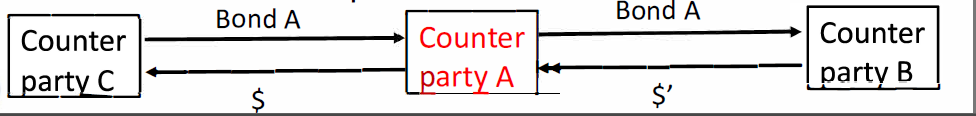
\includegraphics[width=0.5\textwidth]{images/tp.png}
                \caption{tp}
                \label{fig:labe18}
            \end{figure}
        \end{itemize}
    \end{itemize}
\item Repos and Liquidity Management
    \begin{itemize}
    \item Firms balance the costs of funding against the risks of being caught without the financing necessary to survive.
        \begin{itemize}
        \item Repo markets are relatively liquid
        \item Repo borrowing rates relatively low
        \item Short maturities repo is on the less stable side of the funding spectrum, although more stable than short-term, unsecured borrowing like commercial paper.
        \end{itemize}
    \end{itemize}
\end{itemize}




\subsubsection{Risk for entering repo}
\begin{itemize}
\item Counterparty risk: borrower defaults and the collateral's value turns out to be insufficient to cover the loan amount
    \begin{itemize}
    \item Overnight repo and high quality collateral is preferred
    \end{itemize}
\item Liquidity risk: the value of the collateral declining in fire sales
    \begin{itemize}
    \item can be mitigated by haircut
    \end{itemize}
\end{itemize}




\subsubsection{Repo Financing and the Collapse of Bear Stearns}
\begin{itemize}
\item Case brief: During 2006, Bear Stearns decided to reduce short-term unsecured funding and increased the average term of its secured funding during the first half of 2007. Bear Stearns was able to obtain longer term repo facilities of six months or more to finance assets such as whole loans and non-agency mortgage-backed securities. During 2007-2008 crisis, repo lenders began shortening the duration and require higher quality collateral. In the week of March 10, 2008, Bear Stearns suffered a run.
\item Role of repo in the collapses of Bear Stearns:
    \begin{itemize}
    \item The loss of confidence caused three related consequences:
        \begin{itemize}
        \item Withdrew increase: Prime brokerage clients withdrew cash and unencumbered securities at a rapid rate.
        \item Stop renewing repo: Repo lenders declined to roll over repo loans, even when the loans were supported by high-quality collateral such as agency securities.
        \item Capital flight: Result in a rapid flight of capital from the firm that could not be survived.
        \end{itemize}
    \end{itemize}
\end{itemize}




\subsubsection{Repo Financing and the Collapse of Lehman Brothers}
\begin{itemize}
\item Case brief: JPMorgan Chase(JPM) was Lehman's tri-party repo clearing agent. Before Lehman's final week, JPM's tri-party lending to Lehman typically exceeded \$100 billion. JPM had historically not taken any haircuts on its tri-party, intraday advances, but began to do so in early 2008. In Lehman's case, JPM phased in haircuts so as to match, by mid-August 2008, the haircuts posted to overnight repo investors. Finally, Lehman Brothers run out of liquidity to bankrupt.
\item Role of repo in the collapses of Lehman Brothers:
    \begin{itemize}
    \item Over rely on repo: Lehman Brothers relied heavily on shortterm repo as a financing tool.
    \item Haircut increase: When its tri-party repo clearing agent JPM increased haircut, Lehman Brothers could not meet and finally run out of liquidity and finally got bankrupted.
    \end{itemize}
\end{itemize}




\subsubsection{General and special repo rates}
\begin{itemize}
\item Repo trades can be divided into those using general collateral (GC) and those using special collateral or specials.
    \begin{itemize}
    \item GC rates are for overnight repo where any U.S. Treasury collateral is acceptable.
    \item Special rates are for repo being able to borrow cash at a relatively low rate with special securities as collateral.
    \item Special rate is less than the GC rate:
        \begin{itemize}
        \item Special spreads = C rates - Special rates
        \end{itemize}
    \end{itemize}
    
\end{itemize}




\subsubsection{Special spreads and auction cycle}
\begin{itemize}
\item Special collateral:
    \begin{itemize}
    \item Special rates determined by the demand of borrowing that issue to that date relative to the supply available.
    \item On-the-run (OTR) or current issue: The most recently issued bond of a given maturity
        \begin{itemize}
        \item At each maturity, the OTR trades the most special, followed by the old, the double-old.
        \end{itemize}
    \end{itemize}
\item Example: 10- and 30-year U.S. Treasury bonds along with overnight repo rates and spreads as of May 28, 2010
\begin{table}[h]
    \centering
    \begin{tabular}{|l|l|l|l|l|l|}
    \hline
    \rowcolor{lightgray} % 表头行背景色
    \multicolumn{6}{|c|}{General collateral rate 0.23\%} \\ \hline
    \rowcolor{lightgray} % 表头行背景色
    coupon & maturity & Issue date & designation & Repo rate & \textcolor{blue}{spread} \\ \hline
    $3\frac{1}{2}\%$ & 5/15/20 & 5/17/10 & OTR 10yr & 0.09\% & \textcolor{blue}{0.14\%} \\ \hline
    $3\frac{5}{8}\%$ & 2/15/20 & 2/16/10 & Old 10yr & 0.21\% & \textcolor{blue}{0.02\%} \\ \hline
    $3\frac{3}{8}\%$ & 11/15/19 & 11/16/09 & Dbl - Old 10yr & 0.21\% & \textcolor{blue}{0.02\%} \\ \hline
    $4\frac{1}{2}\%$ & 5/15/40 & 5/17/10 & OTR 30yr & 0.18\% & \textcolor{blue}{0.05\%} \\ \hline
    $4\frac{5}{8}\%$ & 2/15/40 & 2/16/10 & Old 30yr & 0.20\% & \textcolor{blue}{0.03\%} \\ \hline
    $4\frac{3}{8}\%$ & 11/15/39 & 11/16/09 & Dbl - Old 30yr & 0.21\% & \textcolor{blue}{0.02\%} \\ \hline
    \end{tabular}
    \end{table}
\item Why OTR securities tend to trade special: liquid is special
    \begin{itemize}
    \item OTR tend to be the most liquid: Extra liquidity of newly issued Treasuries makes them ideal candidates not only for long positions but for shorts.
        \begin{itemize}
        \item Self-fulfilling phenomenon: everyone expects a recent issue to be liquid.
        \end{itemize}
    \end{itemize}
\item Four characteristics of special spreads:
    \begin{itemize}
    \item Quite volatile: spreads are volatile on a daily basis
    \item Quite large: spreads of hundreds of basis points are quite common.
    \item Higher levels over some periods: Special spreads do attain higher levels over some periods rather than others.
    \item Small immediately after auctions and to peak before auctions: The supply of high liquid bond is high after auctions and low before auctions.
    \end{itemize}
\end{itemize}




\subsubsection{Financing Value of a Bond Trading Special in Repo}
\begin{itemize}
\item Financing value of a bond: over the entire life of the bond, borrow cash at its special rate, and invest that cash at the higher GC rate.

\begin{figure}[H]
    \centering
    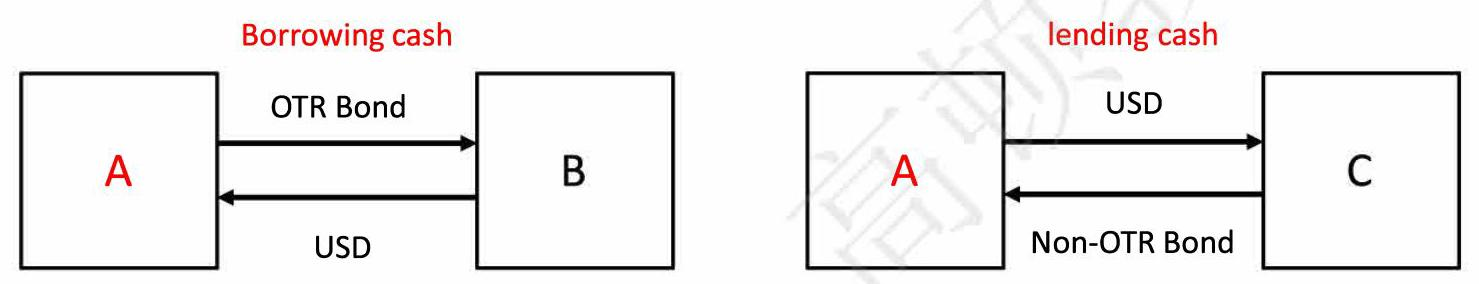
\includegraphics[width=0.5\textwidth]{images/OTR.jpg}
    \caption{OTR}
    \label{fig:labe21}
    \end{figure}
    \begin{itemize}
    \item Financing value of a bond tading special repo = Amount borrowed x special spread x Number of days in Repo borrowing /360 days
    \end{itemize}
    
\item Example
    \begin{itemize}
    \item Assume that the GC rate is 0.25\% and the an OTR bond is currently treated as special securities and will be treated as general collateral from September 30, 2022. The special rate of this bond is only one basis point. Assuming no haircut, What is the financing value per \$100 market value of the bond over the 125 days from the pricing date, May 28, 2022, to September 30, 2022.
    \end{itemize}
\item Answer
    \begin{itemize}
    \item Financing value of a bond tading special repo 125 = 100 X (0.25\% - 0.01 \%) X 360 = 0.083
    \item It means that the financing value is 8.3 cents per 100 dollar market value of the bond.
    \end{itemize}
\end{itemize}


\subsection{Risk Management For changing
Interest Rates Ch18}


\subsubsection{Asset-liability Management Strategy}
\begin{itemize}
\item A balanced approach, also called funds management strategy.
    \begin{itemize}
    \item Manage both assets and liabilities in order to achieve the financial institution's goals.
    \end{itemize}


\begin{figure}[H]
    \centering
    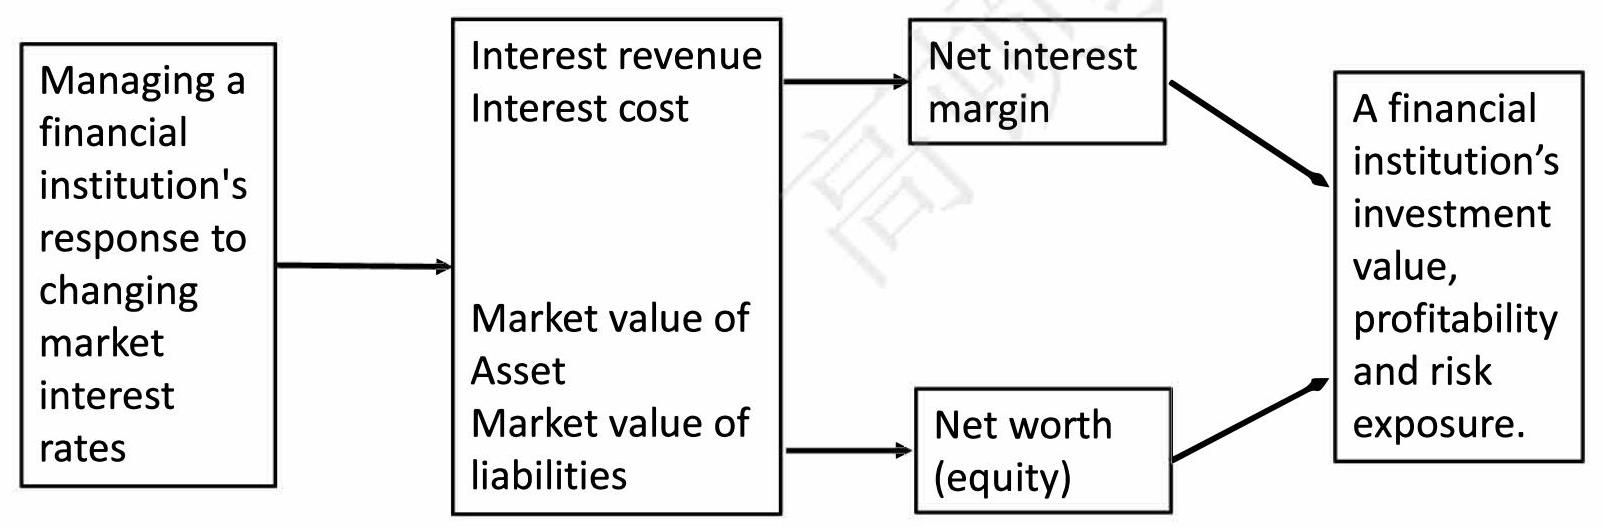
\includegraphics[width=0.5\textwidth]{images/goals.jpg}
    \caption{goals}
    \label{fig:labe22}
    \end{figure}
\end{itemize}




\subsubsection{The impact of interest rate risk}
\begin{itemize}
\item Interest rate risks faced by financial institutions affect both the balance sheet (Net worth) and the statement of income and expenses (Net interest margin).
\item When interest rates change in the financial marketplace:
    \begin{figure}[H]
    \centering
    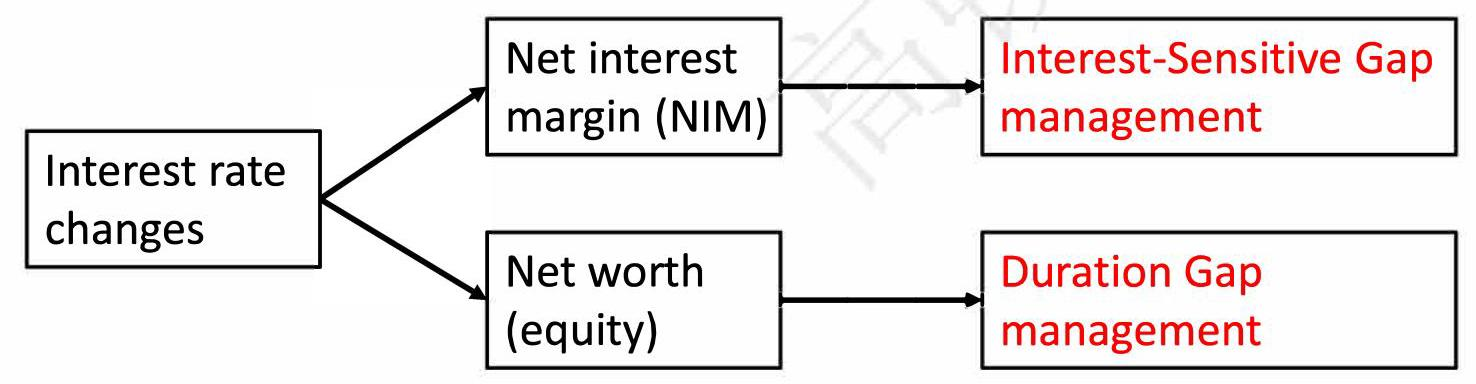
\includegraphics[width=0.5\textwidth]{images/irc.jpg}
    \caption{irc}
    \label{fig:labe22}
    \end{figure}
\end{itemize}




\subsubsection{Net interest margin}
\begin{itemize}
\item Formular: Net interest margin (NIM) = \(\frac{\text{Net interest income}}{\text{Total earning assets}}=\frac{\text{Interest income}-\text{Interest expense}}{\text{Total earning assets}}\)
    \begin{itemize}
    \item Interest income from loans and investments
    \item Interest expense from deposits and other borrowed funds
    \end{itemize}
    
\item Types of assets and liabilities
    \begin{itemize}
    \item Repriceable (interest-sensitive) assets/liabilities
        \begin{itemize}
        \item Variable-rate loans and securities etc.
        \end{itemize}
    
    \item Nonrepriceable assets/liabilities
        \begin{itemize}
        \item Fixed interest rate loans etc.
        \end{itemize}
    
    \end{itemize}
    
\item Net interest income = Total interest income - Total interest cost
    \begin{itemize}
    \item Total interest income = \(Y_{ISA} \times Q_{ISA} + Y_{Non \ ISA} \times Q_{Non \ ISA}\)
    \item Total interest cost = \(Y_{ISL} \times Q_{ISL} + Y_{Non \ ISL} \times Q_{Non \ ISL}\)
        \begin{itemize}
            \item \(Y_{ISA}(Y_{ISL})\): average interest yield (cost) on rate sensitive assets (liabilities)
          \item \(Q_{ISA}(Q_{ISL})\): volume of rate sensitive assets (liabilities)
          \item \(Y_{non \ ISA}(Y_{Non \ ISL})\): average interest yield (cost) on fixed (nonsensitive)assets(liabilities) 
          \item \(Q_{non \ ISA}(Q_{Non \ ISL})\): volume of fixed assets(liabilities)
        \end{itemize}
    \end{itemize}
\item Example
    \begin{itemize}
    \item Suppose the yields on interest rate sensitive and fixed assets average 10\% and 11\%, respectively, while interest rate sensitive and non-interest rate sensitive liabilities cost an average of 8\% and 9\%, respectively. During the coming week the bank holds \$1,700 million in interest rate sensitive assets (out of an asset total of \$4,100 million) and \$1,800 million in interest rate sensitive liabilities. Please calculate the net interest income assuming the equity is zero.
    \item Answer
        \begin{itemize}
        \item Net interest income = 0.1 X 1,700 + 0.11 X (4,100 - 1,700) - 0.08 X 1,800 - 0.09 x (4,100 - 1,800) = \$83 million
        \end{itemize}
    \end{itemize}

\end{itemize}


\subsubsection{Interest-Sensitive Gap management}
\begin{itemize}
\item Interest-sensitive gap(IS GAP) = Interest-sensitive assets （ISA） - Interest-sensitive liabilities(ISL)
\item Relative IS GAP = IS GAP/Size of financial institution
\item Interest Sensitivity Ratio (ISR) = ISA/ISL
\item Asset-sensitive (positive) gap: ISA - ISL > 0
    \begin{itemize}
    \item If interest rates rise, bank's NIM will increase.
    \end{itemize}
\item Liability-sensitive (negative) gap: ISA - ISL < 0
    \begin{itemize}
    \item If interest rates rise, bank's NIM will decrease.
    \end{itemize}
\item Zero interest-sensitive gap: means net interest margin is protected regardless of which way interest rates will go.
    \begin{itemize}
    \item Does not eliminate all interest rate risk.
    \end{itemize}
\item Aggressive GAP management

    \begin{tabular}{|p{5cm}|p{5cm}|p{6cm}|}
        \hline

    \textbf{Expected Changes in Interest Rates (Management's Forecast)} & \textbf{Best Interest-Sensitive GAP Position to Be in:} & \textbf{Aggressive Management's Most Likely Action} \\
    \hline

    Rising market interest rates & Positive IS GAP & Increase interest-sensitive assets\newline Decrease interest-sensitive liabilities  \\
    \hline
     &  &  \\
    Falling market interest rates & Negative IS GAP & Decrease interest-sensitive assets \newline Increase interest-sensitive liabilities \\
    
     \hline

    \end{tabular}   
\item Defensive Interest-Sensitive Gap management
    \begin{itemize}
    \item Set interest-sensitive GAP as close to zero as possible to reduce the expected volatility of net interest income.
    \end{itemize}
\end{itemize}



\subsubsection{Limitation of Interest-sensitive Gap management}
\begin{itemize}
\item Changes inconsistent: Interest rates paid on liabilities tend to move faster that interest rates earned on assets.
\item Basis risk: The interest rates attached to assets of various kinds often change by different amounts and at different speeds than many of the interest rates attached to liabilities.
\item Net worth is not considered.
\end{itemize}



\subsubsection{Duration Gap management}
\begin{itemize}
\item Duration analysis can be used to stabilize , or immunize, the market value of a financial institution's net worth (NW).
\item NW = Assets - Liabilities
    \begin{itemize}
    \item A rise in market rates of interest will cause the market value (price) of both fixed-rate assets and liabilities to decline.
    \end{itemize}
    
\item Price sensitivity to interest rates changes and duration
    \begin{itemize}
    \item \(\dfrac{\Delta P}{P} \approx -D * \dfrac{\Delta i}{(1 + i)}, \quad D: \text{Macauley duration}\)

    \end{itemize}
    
\item \(\Delta NW = \Delta A - \Delta L = \left[-D_A\times\dfrac{\Delta i}{(1 + i)}\times A\right] - \left[-D_L\times\dfrac{\Delta i}{(1 + i)}\times L\right]=-\left[D_A - D_L\times\dfrac{L}{A}\right]\times\dfrac{\Delta i}{(1 + i)}\times A\)
    \begin{itemize}
        \item \(D_A - D_L\): Duration gap
        \item  \(D_A - D_L\times\dfrac{L}{A}\): Leverage - adjusted duration gap
        \item \(D_A\): Dollar - weighted duration of asset portfolio
        \item \(D_L\): Dollar - weighted duration of liability portfolio
    \end{itemize}
    \begin{tabular}{|p{3cm}|c|c|c|}
        \hline
        Leverage - adjusted duration gap & Market interest & The Financial Institution's Net Worth Will: & Value change of Asset/Liability \\
        \hline
        \multirow{2}{*}{Positive} 
        & Rise & Decrease & Assets value $\downarrow\downarrow$ \\
        &  &  & Liabilities value $\downarrow$ \\
        \cline{2 - 4}
        & Fall & Increase & Assets value $\uparrow\uparrow$ \\
        &  &  & Liabilities value $\uparrow$ \\
        \hline
        \multirow{2}{*}{Negative} 
        & Rise & Increase & Assets value $\downarrow$ \\
        &  &  & Liabilities value $\downarrow\downarrow$ \\
        \cline{2 - 4}
        & Fall & Decrease & Assets value $\uparrow$ \\
        &  &  & Liabilities value $\uparrow\uparrow$ \\
        \hline
        \multirow{2}{*}{Zero} 
        & Rise & No change & Assets value $\downarrow$ \\
        &  &  & Liabilities value $\downarrow$ \\
        \cline{2 - 4}
        & Fall & No change & Assets value $\uparrow$ \\
        &  &  & Liabilities value $\uparrow$ \\
        \hline
        \end{tabular}
\item Portfolio immunization strategy
    \begin{itemize}
    \item Leverage-adjusted duration gap equals to zero
    \end{itemize}
    
\item Take chance to maximize the shareholders' position

\begin{tabular}{|p{2.8cm}|p{7cm}|p{7cm}|}
    \hline
    Expected Change in Interest Rates & Aggressive Management's Most Likely Action: & Best Interest-Sensitive GAP Position to Be in: \\
    \hline
    Rates will raise & Reduce \(D_A\) and increase \(D_L\) (moving closer to a negative duration gap) & Net worth increase (if management's rate forecast is correct) \\
    \hline
    Rates will fall & Increase \(D_A\) and reduce \(D_L\) (moving closer to a positive duration gap) & Net worth increase (if management's rate forecast is correct) \\
    \hline
    \end{tabular}
    
\end{itemize}



\subsubsection{Limitation of Duration Gap management}
\begin{itemize}
\item Leverage-adjusted duration gap equals to zero is difficult:
    \begin{itemize}
    \item Hard to find assets and liabilities of the same duration that fit into a financial-service institution's portfolio.
    \end{itemize}
\item Neglect convexity impact:
    \begin{itemize}
    \item Only consider linear relationship
    \item Major changes in interest rate does not apply
        \begin{itemize}
        \item The accuracy and effectiveness of duration gap management decreases when there are major changes in interest rates.
        \end{itemize}
    \end{itemize}
\end{itemize}



\subsection{Illiquid Asset Ch19}



\subsubsection{Characteristics of illiquid markets}
\begin{itemize}
\item Illiquidity: infrequent trading, small amounts being traded, low turnover
\item Most asset classes are illiquid:
    \begin{itemize}
    \item Equity (OTC): a week or more
    \item Municipal bond: annual turnover of less than 10%
    \item Real estate: 4-5 years
    \item Institutional infrastructure: 50 years or longer
    \item Works of art: 40-70 years
    \end{itemize}
    
\item Markets for Illiquid Assets Are Large: the total wealth held in illiquid assets exceeds the total wealth in traditional, liquid stock, and bond markets.
    \begin{itemize}
    \item U.S. residential mortgage market (2012): \$16 trillion
    \item Market capitalization of the NYSE and NASDAQ combined: \$17 trillion
    \end{itemize}
    
\item Investor Holdings of Illiquid Assets: for individual investors, 90\% total wealth is illiquid asset.
    \begin{itemize}
    \item Human capital is the largest and least liquid asset for many individual investors.
    \item High net worth individuals always hold 10-20\% in treasure assets.
    \item University endowments, pension funds, and other institutional investor also allocate much more on this asset kind.
    \end{itemize}
    
\item Liquidity Can Dry Up: In stressed economic periods, liquidity can dry up.
    \begin{itemize}
    \item Illiquidity crises occur regularly because liquidity tends to dry up during periods of severe market distress.
    \end{itemize}
    

\end{itemize}



\subsubsection{Illiquid asset markets}
\begin{itemize}
\item Source of illiquidity: illiquidity arises due to market imperfections

    \begin{itemize}
    \item participation costs: investors must spend money, time, or energy to learn and gain necessary skills (capital, expertise, experience).
    \item Transaction costs: commissions, taxes, due diligence, title transfer, etc.
    \item Search frictions: need to search to find an appropriate buyer or seller.
    \item Asymmetric information: one investor has superior knowledge compared with others so that other investors become reluctant to trade because concerning about fraud.
    \item Price impact: large trades will move markets.
    \item Funding constraints: access to credit is impaired
    \end{itemize}
    
\end{itemize}



\subsubsection{Biases on reported returns}
\begin{itemize}
\item Survivorship bias: results from the tendency of poorly performing funds to stop reporting.
    \begin{itemize}
    \item True illiquid asset returns are worse than the reported data.
    \end{itemize}
\item Reporting bias: occurs when fund never achieves a sufficiently attractive returns, they don't start reporting returns in the first place.
    \begin{itemize}
    \item Overestimate the expected return
    \end{itemize}   
\item Infrequent trading:
    \begin{itemize}
    \item Return volatilities are underestimated.
    \item Correlations with market (other assets) and betas are underestimated.
    \item Returns for these infrequently traded assets are smoothed.
    \end{itemize}
    \begin{figure}[H]
        \centering
        \includegraphics[width=0.5\textwidth]{images/sampling.jpg}
        \caption{sampling bias}
        \label{fig:labe22}
        \end{figure}
\item Selection bias: Asset values and returns tend to be reported when they are high. Sample selection bias results in overestimated expected returns and underestimated risk as measured by beta and the standard deviation of returns.


    \begin{itemize}
    \item Buildings: many sellers postpone sales until property values recover.
    \item Private equity: The venture capitalist tends to sell a small company, when the company's value is high and the transaction is recorded.
    \end{itemize}

\item \begin{tabular}{|c|c|}
    \hline
    Biases & Results in \\
    \hline
    Survivorship bias \newline Reporting bias & Overestimated expected returns \\
    \hline
    \multirow{3}{*}{\makecell{Infrequent trading $\rightarrow$ \\ smoothed data}} & Underestimated standard deviation \\
    & Underestimated correlation with market (beta) \\
    & Overestimated return autocorrelation \\
    \hline
    Selection bias & \makecell{Overestimated expected returns \\ Underestimated risk ($\sigma$, beta)} \\
    \hline
    \end{tabular}

\end{itemize}




\subsubsection{Illiquidity risk premiums}
\begin{itemize}
\item Illiquidity risk premiums: compensate investors for the inability to access capital immediately.
    \begin{itemize}
    \item Allocation across asset classes (e.g. real estate)
    \item Choose securities within an asset class that are more illiquid
    \item Act as market maker at the individual security level
    \item Rebalancing
    \end{itemize}
    \begin{figure}[H]
        \centering
        \includegraphics[width=0.5\textwidth]{images/liquidreturn.jpg}
        \caption{liquidreturn}
        \label{fig:labe22}
        \end{figure}

\end{itemize}





\subsubsection{Illiquidity risk premiums across asset classes}
\begin{itemize}
\item Conventional view: there is a reward to bearing illiquidity across asset classes. It may not be possible to generate illiquidity risk premiums across illiquid asset classes.
    \begin{itemize}
    \item Illiquidity biases: reported data on illiquid assets cannot be trusted (survivorship, infrequent trading, selection bias).
    \item Ignores risk: illiquid asset classes contain far more than just illiquidity risk (hedge fund and private equity fund). After adjusting for risk, these illiquid asset classes will be less compelling.
    \end{itemize}
    
\item There is an evidence of large illiquidity risk premiums within asset classes.
    \begin{itemize}
    \item Within asset classes: take long positions in illiquid assets and short positions in liquid ones.
        \begin{itemize}
        \item U.S. Treasuries: on-the-run/off-the-run
        \item Corporate Bond: Larger bid-ask spreads and infrequent trading led to higher yields in corporate bond markets.
        \item Equity: many illiquidity variables predict returns in equity markets, with less liquid stocks having higher returns.
        \end{itemize}
    \end{itemize}
    
\item Why illiquidity risk premiums manifest within but not across asset classes?
    \begin{itemize}
    \item Limited integration across asset classes: investors put asset classes into different silos and rarely treat them as a whole.
    \end{itemize}
    
\end{itemize}



\subsubsection{Liquidity providing activities}
\begin{itemize}
\item Market making: A market maker supplies liquidity by acting as an intermediary between buyers and sellers.
    \begin{itemize}
    \item Liquidity provision is costly: Investors transacting with the market maker pay the bid-ask spread.
    \end{itemize}
    
\item Rebalancing: the simplest way to provide liquidity, as well as the foundation of all long-horizon strategies.
    \begin{itemize}
    \item Rebalancing forces asset owners to buy at low prices when others want to sell.
    \item Since rebalancing is counter-cyclical, it supplies liquidity.
    \end{itemize}
    
\end{itemize}



\subsubsection{Portfolio choice with illiquid assets}
\begin{itemize}
\item Investors face many considerations on how much of their portfolios to devote to illiquid assets:
    \begin{itemize}
    \item Investors have different horizons
    \item Illiquid market don't have tradable indices
    \item Talented active portfolio managers are needed (agency issues)
    \item How to evaluate and monitor portfolio managers
    \end{itemize}
\item Practice
    \begin{itemize}
    \item For a portfolio of illiquid assets, hedge fund managers often have considerable discretion in portfolio valuation at the end of each month and may have incentives to smooth returns by marking values below actual in high-return months and above actual in low-return months. Which of the following is not a consequence of return smoothing over time?
    
    A. Higher Sharpe ratio

    B. Lower volatility

    C. Higher serial correlation

    D. Higher market beta
    \item Answer: D
    \item 解析:根据题意，可以得知数据出现被平滑化，被平滑的数据会出现，波动率被低估，自相关系数被高估，市场B被低估的效果。因此，A，B，C三个选项是平滑数据导致的结果不符合题意，D选项符合题意，为正确选项。
    \end{itemize}
    
\end{itemize}



